\begin{abstract}
This document is an electricity primer that begins with first principles.
\end{abstract}

\section{Electricity}

The electromagnetic interaction is one of the four fundamental forces
of nature.

Historically, electricity and magnetism were conceptualized as being
different but connected, which is reflected in classical classroom
treatments that treat electricity and magnetism as two different
phenomena that interact. In fact, magnetism is a relativistic
consequence of the movement of electric charge.

For our purposes the classical phenomenological description is more
than adequate.

\subsection{Electrostatics}

\subsubsection{Charge Carriers and Continuity}

In this description, charge is treated as a continuously variable
scalar quantity with two types: ``positive'' and ``negative''. Like
charges repel each other and unlike charges attract each other. The
S.I. unit of charge is the \emph{coulomb}\footnote{S.I. units are
  treated as common nouns and are \emph{not} capitalized other than at
  the beginning of a sentence.}, symbol \emph{C}\footnote{The symbols
  for S.I. units named after persons, and \emph{only} those S.I units,
  are \emph{always} capitalized.}.

In the best current theory, charge is ultimately carried by a number
of \term{elementary particles}\footnote{Specifically electrons, muons,
  tau leptons, quarks, and their respective antiparticles.} but for
almost all practical purposes in electrical and electronic
engineering, the only real charge-carrier is the negatively charged
electron. There are a few circumstances where positive charge occurs
in practice --- as ions in plasma and in solutions in electrochemistry
--- but outside of a handful of exceptions, when we talk about a
positive charge in electrical and/or electronic engineering, it's a
convenient fiction or an abstraction: what's really going on is all
about electrons.

An electron carries a charge of $\approx
-1.6\times10^{-19}\unit{C}$. Compared to the amounts of charge we deal
with in practice, this is so minuscule that there's no problem with
the assumption of continuity.

\subsubsection{The Coulomb Force}

Charges exert a force on each other, sometimes called the
\term{Coulomb force} to distinguish it from other forces. 

The force, in newtons (\unit N), experienced by a charge, $Q_1$, at a
fixed position, $\vec{r}$, relative to another charge, $Q_0$, at the
origin, is given by an inverse-square law much like Newton's Law of
Gravitation, called \term{Coulomb's Law}:

\begin{equation}
\label{eqn:coulombs}
F(\vec{r}) = \frac{1}{4\pi\epsilon}\frac{Q_0 Q_1}{|\vec{r}\,|^2} \hat{r} \qquad\bunit{N}{C}
\end{equation}

Where $\hat{r}$ is the unit-vector from the origin to $Q_1$ and
$\epsilon$ is the \term{permittivity} of the ``universe'' where the
two charges sit. As you might expect, $Q_0$ experiences the same
force, but in the opposite direction, $-\hat{r}$.

Permittivity can be thought of as a property of a material that says
how effectively it blocks the electric force: the higher the
permittivity, the lower the Coulomb force experienced by the two
charges. We won't have much need for discussing permittivity, but just
to give you an idea of its magnitude, the \term{permittivity of free
  space} or \term{vacuum permittivity} is about 8.85\unit{F}{m}
(farads\footnote{more about farads later} per meter).

Note that, in general, permittivity is a tensor quantity, since many
materials have different permittivities in different directions: think
of materials like mica or graphite.

\subsubsection{Linear Superposition}

Electrical charge obeys the principle of linear superposition. That is
to say that the total force experienced by a charge, $Q_2$, due to two
other charges, $Q_1$ and $Q_0$, is just the vector sum of the forces
that $Q_2$ would feel due to each of the other charges considered
individually.

\subsubsection{Electric Field}

The \emph{electric field} due to some configuration of charges is just
the force per unit charge that would be experienced by a positive
charge due to that configuration of charges according to Coulomb's
Law. Not surprisingly, the E-field has units of newtons (force) per
coulomb (charge) and is a vector quantity.

The E-field (in \unit{N}{C}) experienced by a charge, $Q_1$, at a
position $\vec{r}$ relative to another charge, $Q_0$, at the origin
follows directly from Coulomb's Law (above):

\begin{equation}
\label{eqn:efield}
E(\vec{r}) = \frac{1}{4\pi\epsilon}\frac{Q_0}{|\vec{r}\,|^2} \hat{r} = \frac{F(\vec{r})}{Q_1} \qquad\bunit{N}{C}
\end{equation}

You can probably imagine that if you placed a positive charge on one
of the black \term{field lines} of Figure~\ref{fig:positive}, it
would be accelerated away from the charge shown in the center along
the same field line. The further away it gets, the weaker the
accelerating force becomes, so while the field lines indicate the
direction a positive charge will move, how close together the field
lines are is an indication of the strength of the field.

\begin{figure}[H]
  \centering
  \subfigure[Positive Charge]{%
    \label{fig:positive}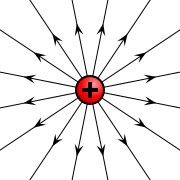
\includegraphics[width=\twowide]{positive}
  }\hskip4em
  \subfigure[Negative Charge]{%
    \label{fig:negative}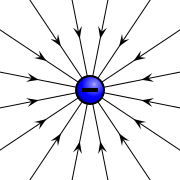
\includegraphics[width=\twowide]{negative}
  }
  \caption{Electric Field Due to An Isolated Point Charge}
  \label{fig:onecharge}
\end{figure}

Electro\emph{static} fields are conservative\footnote{As we will see,
  things change a little for time-varying electric fields.}. In other
words, if you moved a charge from a point, $a$, to another point, $b$,
in an electrostatic field, the amount of work you would have to do is
independent of the path, $\ell$, taken from $a$ to $b$. Moreover, if
you moved a charge through a closed loop from $a$ back to $a$ again,
you would do no net work, no matter how big or small the loop or how
circuitous its path.

\begin{equation}
\oint_\ell \vec{E}\cdot\dee{\vec{\ell}} = 0
\end{equation}
or
\begin{equation}
\curl{E} = 0
\end{equation}

\subsubsection{Electric Potential}

Mathematically, a conservative vector field is the gradient of some
scalar field:
\begin{equation}
\vec{E} = -\grad\phi \qquad\bunit{N}{C}
\end{equation}
or
\begin{equation}
\phi = -\int \vec{E}\cdot\vec{\dee\ell} \qquad\bunit{N\cdot m}{C}
\end{equation}

The unit of newton-meters, or joules\footnote{Recall that the joule is
  \emph{defined} as the work done when an object is moved one meter
  against a force of one newton.}, per coulomb is called the
\term{volt}:
\begin{equation}
V = \unit{N\cdot m}{C} = \unit{J}{C}
\end{equation}

Figure~\ref{fig:dipole} shows the $\vec{E}$-field and equipotential
contours of an electrostatic dipole. Note that the $\vec{E}$-field
lines are everywhere perpendicular to the isolines of electric
potential.

Conventionally, the units of electric field are given as volts per
meter, which is equivalent to the earlier units of newtons per
coulomb:

\begin{equation}
\unit{V}{m} = \frac{\unit{N\cdot m}{C}}{\unit{m}} = \unit{N\cdot m}{C}\cdot\unit{1}{m} = \unit{N}{C}
\end{equation}
%\int_a^b \vec{E}\cdot\dee{\vec{\ell}} = \phi|_b - \left.\vec{E}\right|_a

\begin{figure}[ht]
  \centering
  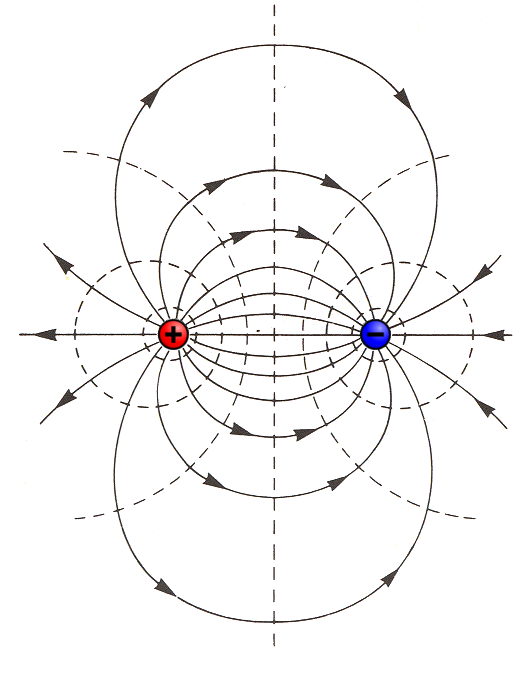
\includegraphics[width=\onenarrow]{potential-dipole}
  \caption{Field Lines and Equipotential Contours of a Dipole}
  \label{fig:dipole}
\end{figure}

So the electric potential at a point, $p$, in an electric field is the
work done (or yielded) by moving a point charge, $Q$, from where the
E-field is zero (infinitely far away from any charges) to that point
per coulomb of $Q$'s charge.

\subsubsection{Electric Potential Difference}

As for other scalar potential fields, we're generally more interested
in differences in potential than in absolute potentials. The electric
potential difference, colloquially called \term{voltage}, is
(unsurprisingly) just the difference in electric potential between two
points.

So, {\bf ``voltage'' is a measure of electric potential energy,
  measured in units of energy per unit charge or joules per
  coulomb}. This is analgous to gravitational potential in joules per
  unit mass, or pressure in joules per unit volume.

Consider, for example, the familiar equation for gravitiational
potential energy, $E_\mathrm{GP} = mgh$. This can be viewed as the
gravitational potential difference of an object of mass, $m$, on the
ground and the same object raised to a height, $h$. The analog of
``voltage'', then, would be the $gh$ product, which should have units
of joules per kilogram (by analogy with joules per coulomb), and so it
does:

\begin{equation}
g\bunit{m}{s^2}\cdot h\bunit{m} = gh\left[\unit{m^2}{s^2}\cdot\unit{kg}{kg}\right] = gh\left[\unit{kg\cdot m^2}{s^2}\cdot\unit{1}{kg}\right] = gh\bunit{J}{kg}
\end{equation}


\subsubsection{Charge Distributions}

Suppose you did that old trick where you rub your hair with a balloon,
then hold it a few inches away from your head so it lifts your hair
up\footnote{Assuming that your hair is fine enough, long enoug, and
  the relative humidity is low enough}.

On the head side of the balloon, there is a surface distribution of
negative charge. Your hairs, on the other hand, have a net positive
charge. The unlike charges attract, and your hair is lifted toward the
balloon. The like charges on the hairs repel each other, and the hairs
spread out.

The point is that, in classic electromagnetic theory, you can have
arbitrary surface and volume distributions of charge, not just point
charges.


\subsubsection{Current}

The macroscopic net movement of charge is called \term{current}.

In a copper wire, electrons are constantly whizzing around the nuclei
of the copper atoms, but we don't call this a current: we're only
interested in \emph{net} movement of charge at, at least, a
super-atomic level. In semiconductors, admittedly, the scales where we
talk about current can be very small, but we're still concerned with
net movement.

Not surprisingly, current is measured in units of charge per unit
time, or coulombs per second. A coulomb per second is called an
\term{amp\`ere}.

Strictly speaking, it's the other way around: the amp\`ere is an SI
fundamental unit and the coulomb, or amp\`ere-second, is the derived
unit.

\subsubsection{Ohm's Law}

So what, one might reasonably ask, is the relationship between
potential difference and current in a medium that permits charge to
move?

Intuitively, one would expect that the greater the potential
difference, the greater the amount of current that will flow.

But, as you might expect, it's also dependent on the medium: some
media impede the flow of charge-carriers --- electrons --- more than
others. As a bulk material property, this is called
\emph{resistivity}. As a property of an object, such as a circuit
element or a cable, it is called \emph{resistance}.

If an object has a potential difference of $V_\mathrm{R}$ volts across
its ends, and that causes a current of $I_\mathrm{R}$ amp\`eres to
flow, then the object's resistance, $R$, is given by:

\begin{equation}
R = \frac{V_\mathrm{R}}{I_\mathrm{R}} \qquad\left[\unit{V}{A}=\unit{\Omega}\right]
\end{equation}

Simple, eh?

The unit of volts per amp\`ere has a special name, the \term{ohm},
symbol \unit{\Omega}.


\section{Electrodynamics}




\end{document}


